%\documentclass{article}
%\usepackage{xcolor}
%\usepackage[linesnumbered,ruled,vlined]{algorithm2e}
%\usepackage{amsmath}

%\title{Algorithms}
%\author{Francis}

%%% Coloring the comment as blue
\newcommand\mycommfont[1]{\footnotesize\ttfamily\textcolor{blue}{#1}}
\SetCommentSty{mycommfont}

\SetKwInput{KwInput}{Input}                % Set the Input
\SetKwInput{KwOutput}{Output}              % set the Output


%\begin{document}
	%\maketitle
%%%%%%%%%%%%%%%%%%%%%%%%%%%%%%%%%%%% INTRO 1 %%%%%%%%%%%%%%%%%%%%%%%%%%%%%%%%%%%%%%%%%%%%
	
	\hl{The Constructive Heuristic for the Aircraft Recovery Problem (CHARP) is based in constraint satisfaction problems (CSP) and consists of two heuristics, that perform a pincer movement over two subsets of the search space. We define two parameters consisting of an upper bound and lower bound. If the search space size is greater than the upper bound the model uses the upper heuristic, whereas if the search space is lower than the lower bound the model uses the lower heuristic.
	}
	 Given the original aircraft rotation and a set of disruptions, the objective of the CHARP is to create a new combination of aircraft routings during the RTW to minimize the total cost of recovery. 
	\hl{In the next sections we describe in detail the algorithms that compose the CHARP, namelly in Section} \ref{sec:newFlightsAlgo} \hl{the algorithm that creates the flights in the presence of flight or aircraft disruption, in Section} \ref{sec:feasVer} \hl{ the algorithm that checks the rotation's feasibility, in Section} \ref{sec:flightDomains} \hl{the algorithm that computes the domains for each flight, in Section} \ref{sec:lowerHeuristic} \hl{the lower heuristic, in Section} \ref{sec:upperHeuristic} \hl{the upper heuristic, in Section} \ref{sec:backtracking} \hl{ the backtracking algorithm, in Section} \ref{sec:taxiFlights} \hl{the taxi flights algorithm, and finally in Section} \ref{sec:charp} \hl{the CHARP algorithm.}


	\subsection{New Flights Algorithm} \label{sec:newFlightsAlgo}
	The algorithm starts by initializing the particular data instance after which it will loop through each aircraft and their rotations. After initializing the rotation the algorithm checks the rotation for cancelled flights or aircraft breakdown periods that also lead to flight cancellation. If these disruptions exist the algorithm will then create new flights.
	
	
	
%%%%%%%%%%%%%%%%%%%%%%%%%%%%%%%%%%%%%%%% ALGORITHM 1 %%%%%%%%%%%%%%%%%%%%%%%%%%%%%%%%%%	
	Algorithm \ref{algo:newFlightAircDisr} describes the creation of new flights. The algorithm receives as inputs the aircraft rotation, the distance set, the maximum flight number, the aircraft breakdown period and the end time of the recovery window. The algorithm will return the aircraft rotation with the new flight and the updated maximum flight number. This algorithm starts by initializing two sub-rotations containing available flight slots, the cancelled flights and the starting time from which new flights can be created. The algorithm will afterwards loop through the new flight slots and cancelled flights and calculate the departure time and the flight time (line 6). If the departure time added to the flight time of the new flight over shoots the end time of the recovery time window the loop breaks and the algorithm returns the rotation with the new flights and the number of the last flight. Else, the flight number is incremented a and the new flight slot is updated (lines 11 to 15). Finally the algorithm checks if the new flight's arrival time added with the transit time overshoots the end time of the recovery time window. If true the algorithm breaks the loop  and returns the rotation with the new flights and the number of the last flight. An identical algorithm can be derived from \ref{algo:newFlightAircDisr} by simply allocating the new flight slots to those that were cancelled due to flight disruption.\\
	
	\begin{algorithm}[H]
		\DontPrintSemicolon
		
		\KwInput{$ \sigma_p, \Delta, M, \mathcal{B}_b, RTW_e$}
		\KwOutput{$ \sigma_p, M$}
		$\sigma^n_p \gets$ List of available new flights in $\sigma_p$ \\
		$\sigma^c_p \gets$ List of cancelled flights in $\sigma_p$ \\
		$start \gets$ end time of aircraft disruption $\mathcal{B}_b$\\
		\For{ $\sigma^n_{p}(i), \sigma^c_p(i)$ in $\sigma^n_p, \sigma^c_p$}
		{
			\If{$i \neq 0$} { $start \gets \sigma^{na}_p(i-1)  + t_{rp}$}
			$\delta_{of} \gets \Delta(\sigma^{co}_p(i), \sigma^{cf}_p(i))$\\
			\If{$start + \delta_{of}> RTW_e$}{break}
			$M \gets M + 1$\\
			$\sigma^n_p(i) = M$\\
			$\sigma^{nd}_p(i) \gets start$ \\
			$\sigma^{no}_p(i) \gets \sigma^{co}_p(i)$\\
			$\sigma^{na}_p(i) \gets start + \delta_{of}$\\
			$\sigma^{nf}_p(i) \gets \sigma^{cf}_p(i)$\\
			\If{$\sigma^{na}_p(i) + t_{rp} > RTW_e$}{break}	
		}
		return $\sigma_p, M$
		\caption{New flights from aircraft disruption}
		\label{algo:newFlightAircDisr}
	\end{algorithm}


%%%%%%%%%%%%%%%%%%%%%%%%%%%%%%%%%%%%%%%% ALGO 2 %%%%%%%%%%%%%%%%%%%%%%%%%%%%%%%%%%	
\subsection{Feasibility Verification Algorithm} \label{sec:feasVer}
The next step uses algorithm \ref{algo:feas} consists in traversing the rotation to find  if the following five constraints are being respected:\\

\begin{itemize}
	\item Flight schedule continuity.\\
	\item Transit or turnround time between consecutive flights.\\
	\item Departure and arrival airport capacity.\\
	\item Aircraft arrive on time for maintenance.\\
\end{itemize}

The algorithm receives as inputs the aircraft rotation and the airport set.   The algorithm will  verify the infeasibilities in the rotation regarding transit time, airport departure and arrival capacity, and maintenance (lines 1 to 5). In line 6 the algorithm concatenates all the infeasibility sets in a single set and if the latter is not empty it returns the rotation and the index of the first infeasbility. Else, if the rotation is feasible the algorithm returns an empty set and -1. Consequently, the rotation will be add to the recovery solution, the departure and arrival airport capacity is updated and the algorithm and moves to the next aircraft.

%%%%%%%%%%%%%%%%%%%%%%%%%%%%%%%%%%%%%%%% ALGORITHM 2 %%%%%%%%%%%%%%%%%%%%%%%%%%%%%%%%%%	


	\begin{algorithm}[H]
		\DontPrintSemicolon
		\KwInput{$ \sigma_p, \mathcal{A}$}
		\KwOutput{$ \sigma_p, index$}
		%new aircraft flights
		$inf1 \gets continuity(\sigma_p)$\\		%continuity
		$inf2 \gets tt(\sigma_p)$\\ 		%tt
		$inf3 \gets dep(\sigma_p, \mathcal{A})$\\%dep
		$inf4 \gets arr(\sigma_p, \mathcal{A})$\\%arr
		$inf5 \gets maint(\sigma_p)$\\ %maint
		$inf \gets inf1 \cup inf2 \cup inf3 cup inf4 \cup inf5$\\
		\If {$inf \ne \{\}$} %if infeasible
		{
			$index \gets min(infList)$\\
			return $\sigma_p, index$\\
		}
		\Else{return $[], -1$ }%if feasible
		\caption{Feasibility verification}
		\label{algo:feas}
	\end{algorithm}

%%%%%%%%%%%%%%%%%%%%%%%%%%% ALGO 3 %%%%%%%%%%%%%%%%%%%%%%%%%%%%%%%%%%%%%%%%%%%%%%%%%%%%%%%

\subsection{Flight Domains Algorithm} \label{sec:flightDomains}
Starting at the first infeasible flight in the infeasible rotation the next step of the recovery procedure consists of an algorithm that searches for each flight, of this part of the rotation, the domain where it is possible to depart and land without breaching airport departure and arrival capacity constraints. This search is done incrementally and it will allow to delay the rotation’s flights. Added to the latter, and with the exception of those flights that are already subject to a disruptive delay, the algorithm also adds the option to cancel the flight as a delay valued -1. To implement this procedure, algorithm \ref{algo:flightDomains} receives as inputs the infeasible rotation, the airport capacity, the maximum amount of delay and the delay increment. After initializing the variables to save the rotation's flight domains, singletons and size of the search space (line 1 to 3) the algorithm loops through the rotation to compute and retrieve their respective values. The flight domain is initialized in line 5 and if it has been disrupted its domain assumes a single value of zero thus becoming a singleton (line 7). If the singleton makes the recovery infeasible by breaking the airport capacity constraint it will be added to the singleton list and the algorithm loops to the next flight in the rotation (line 8 and 9). If the flight departs outside the recovery the algorithm will simply return the flight ranges, the singleton list and the total number of combinations. If the flight is neither disrupted or departs outside the recovery time window then the algorithm adds the cancellation option. Afterwards it will loop incrementally through the range of delay values starting at zero and add any of them that make the flight feasible (lines 14 to 20). In lines 21 and 22 the algorithm adds the domain to the flight domains dictionary and updates the number of combinations. \\

%%%%%%%%%%%%%%%%%%%%%%%%%%%%%%%%%%%% ALGORITHM 3 %%%%%%%%%%%%%%%%%%%%%%%%%%%%%%%%%%%%%%%%%%	
		\begin{algorithm}[H]
		\DontPrintSemicolon
		\KwInput{$ \sigma_p, \mathcal{A}, maxDelay, delayIncrement$}
		\KwOutput{$flightDomains, singletonList, totalCombos$}
		$flightRanges \gets \{\}$\\
		$singletonList \gets \{\}$\\
		$totalCombos \gets 1$\\
		\For{ $\sigma_p(i)$ in $\sigma_p$ }
		{
			$domain \gets \{\}$\\
			\If{$\sigma_p(i) \cap \mathcal{D}_d \ne \{\}$}{
				$domain \gets domain \cup \{0\}$\\
				$checkSingleton(\sigma_p(i), \mathcal{A}, singletonList)$\\
				continue\\}
			\If{$(\sigma^d_p(i) < RTW_s) \lor (\sigma^d_p(i) > RTW_e)$}
				{return $flightRanges, singletonList, totalCombos$\\}
			$domain \gets domain \cup \{-1\}$\\ %cancel the flight
			\For{$delay$ in $range(0, maxDelay, delayIncrement)$}{
				$dep \gets \sigma^d_p(i)$\\
				$arr \gets \sigma^a_p(i)$\\
				$ dep \gets dep + delay$\\
				$ arr \gets arr + delay$\\
				$ \sigma^\prime_p(i) \gets \sigma_p(i, dep, arr)$\\
				\If{$(dep(\sigma^\prime_p(i), \mathcal{A}) = []) \land (arr(\sigma^\prime_p(i), \mathcal{A}) = [])$}{
					$domain \gets domain \cup delay$
				}
			}
			$flightDomains[\sigma_p(i)] \gets domain$\\
			$totalCombos \gets totalCombos * |domain|$\\
		}
		return $flightRanges, singletonList, totalCombos$
		\caption{Find flight domains}
		\label{algo:flightDomains}
	\end{algorithm}

Each flight domain will be coded in a dictionary, using the flight number and date as the key, and a vector with all the possible delay as the value:

	
	{\texttt{\footnotesize \\ \\ \{'286802/03/08': [-1, 0],
			'720201/03/08': [-1, 60, 120, 180, 240, 360, 420],
			'720701/03/08': [-1, 0, 120, 180, 360, 420],
			'730801/03/08': [-1, 0, 240, 300],
			'737502/03/08': [-1, 0, 60, 120, 180, 240],
			'742002/03/08': [-1, 0, 120],
			'744002/03/08': [-1, 0]\}}}\\ \\	

	
Each vector consists of the domain values that the flight can assume, and the search space is obtained by computing the Cartesian product between all the vectors. Any infeasible rotation has a search space that consists of a matrix whose columns are the flights and the rows are the possible values each flight can have.\\
 	
$\begin{bmatrix}
	-1	&  -1	&  -1	& ...	&  -1 &	  -1 &	-1\\
	-1	&  -1	&  -1	& ...	&  -1 &	  -1 &	0\\
	-1	&  -1	&  -1	& ...	&  -1 &	   0 &	-1\\
	...	&		&		&       &     &      &      \\    	
	420	& 420	& 300	& ...	& 120 &	 180 &	0\\
	420	& 420	& 300	& ...	& 120 &	 240 &	-1\\
	420	& 420	& 300	& ...	& 120 &	 240 &	0\\
\end{bmatrix}$
\newline
\newline
\newline
%%%%%%%%%%%%%%%%%%%%%%%%%%%%%%%%%%%%%%%%%% ALGO 4 %%%%%%%%%%%%%%%%%%%%%%%%%%%%%%%%%%%%%%%%%%%%
\subsection{Lower Heuristic Algorithm} \label{sec:lowerHeuristic}

In our experiments we found that the number of rows varies between the order of magnitude $10^3$ to $10^{12}$, hence it is not possible a unique approach to find feasible solutions. To tackle the two distinct situations the algorithm uses a lower heuristic for the lower bound of the search space and an upper heuristic to handle the upper bound of the search space.\\
The lower bound is initialized at $4 \times 10^4$ by default, and the lower heuristic loops through every row of the of the matrix in order to find the optimal solutions that minimize the number of cancelled flights and the total amount of delay. Algorithm \ref{algo:lowerHeuristic} receives as inputs the rotation, the index of the first infeasibility and the search space in the form of a matrix. The algorithm will recover the infeasible rotation and will output the recovered one. It starts by initializing the best solution in line 1 and henceforward it will loop through the search space to find its value. In lines 3 and 4 for the algorithm sums the the cancelled flights and the total amount of delay for each row of the matrix and in line 5 it assigns them to the new solution. The algorithm compares the new solution with the best one and if the new one is not better it will iterate (lines 6 to 10). Based on the values coded in the row, in line 11 the algorithm creates the new rotation by cancelling or delaying flights. Afterwards if the row creates a new feasible solution the best solution is updated (lines 12 to 18). After traversing the entire search space the algorithm updates the aircraft rotation with the optimal solution and returns it (lines 19 and 20).\\
%%%%%%%%%%%%%%%%%%%%%%%%%%%%%%%%%%%%%%%%%%%% ALGORITHM 4 %%%%%%%%%%%%%%%%%%%%%%%%%%%%%%%%%%%
\begin{algorithm}[H]
	\DontPrintSemicolon
	
	\KwInput{$ \sigma_p, index, matrix $}
	\KwOutput{$\sigma^\prime_p$}
	$bestSol \gets \{\}$\\
	\For{ $row$ in $matrix$ }
	{
		$noCancel \gets \sum_{i} row(i),$ if $row(i) = -1$;\\
		$totalDelay \gets \sum_{i} row(i),$ if $row(i) \ne -1$	\\
		$newSol \gets \{noCancel, totalDelay, row\} $\\
		\If{$bestSol \ne \{\} $}{
			\If{$newSol[0] < bestSol[0]$}{continue}
			\If{$(newSol[0] = bestSol[0]) \land (newSol[1] > bestSol[1])$}{continue}
		}
		$\sigma^\prime_p \gets \sigma_p(row)$\\
		\If{$continuity(\sigma^\prime_p) \ne \{\}$}{continue}		%continuity
		\If{$tt(\sigma^\prime_p) \ne \{\}$}{continue} %tt
		\If{$maint(\sigma^\prime_p) \ne \{\}$}{continue} %maint
		$bestSol \gets newSol$\\
		
	}
	$\sigma^\prime_p \gets \sigma_p(bestSol[2]) $\\
	return $\sigma^\prime_p$
	\caption{Lower heuristic}
	\label{algo:lowerHeuristic}
\end{algorithm}


%%%%%%%%%%%%%%%%%%%%%%%%%%%%%%%%%%%%% ALGO 5 %%%%%%%%%%%%%%%%%%%%%%%%%%%%%%%%%%%%%%%%%%%%%%%%
\subsection{Upper Heuristic Algorithm} \label{sec:upperHeuristic}

The upper heuristic's upper bound is initialized at $3 \times 10^{12}$ by default. This heuristic  decomposes the rotation into sub-rotations with a search space size lower than the lower bound defined for the lower heuristic. The algorithm loops through every sub-rotation until it finds a feasible solution for the entire rotation. Although this procedure does not return an optimal solution, it can find feasible solutions in a reasonable computing time. Algorithm \ref{algo:upperHeuristic} receives as inputs the infeasible rotation, the index of the first infeasibility and flight domains. On line 1, the lower index of the sub-rotation is initialized with the value of the index of the first infeasibility. I line 2 the algorithm uses a sub-routine that computes the upper index for the sub-rotation that will be recovered and extracts the corresponding flight domains. In line 3 the algorithm computes the search space and  in line 4 reduces the flight domains to the un-recovered part of the inputted rotation. From line 5 to 29 the algorithm will loop through every sub-rotation, recovering each one of them. With the exception of maintenance check, the algorithm finds the best solution to recover the sub-rotation using a similar method as in the lower heuristic (lines 7 to 21). In line 22 the part between the lower and the upper index of the inputted rotation is updated with the best solution. If the upper index equals the size of the inputted rotation this means the recovery procedure is over and it returns the recovered rotation (lines 23 and 24). Else, the algorithm assigns the upper index to the lower index, computes the new upper index and new partial flight domains, computes the search space and the remaining flight domains.

%%%%%%%%%%%%%%%%%%%%%%%%%%%%%%%%%%%%% ALGORITHM 5 %%%%%%%%%%%%%%%%%%%%%%%%%%%%%%%%%%%%%%%%%%%

\begin{algorithm}[H]
	\DontPrintSemicolon
	
	\KwInput{$ \sigma_p, index, flightDomains$}
	\KwOutput{$\sigma_p$}
	$lIndex \gets index$ \\
	$uIndex, partialFlightDomains \gets upperIndex(lIndex, \sigma_p, flightDomains)$ \\
	$matrix \gets product(partialFlightDomains.values())$ \\
	$removeFlightDomains(flightDomains, \sigma_p(i) \forall i \in [uIndex, |\sigma_p|])$\\
	\While{True}{
		$bestSol \gets \{\}$\\
		\For{$row$ in $matrix$}{
			$noCancel \gets \sum_{i} row(i),$ if $row(i) = -1$;\\
			$totalDelay \gets \sum_{i} row(i),$ if $row(i) \ne -1$	\\
			$newSol \gets [noCancel, totalDelay, row] $\\
			\If{$bestSol \ne \{\} $}{
				\If{$newSol[0] < bestSol[0]$}{continue}
				\If{$(newSol[0] = bestSol[0]) \land (newSol[1] > bestSol[1])$}{continue}
			}
			$\sigma^\prime_p(i) \gets \sigma_p(row)$\\
			\If{$continuity(\sigma^\prime_p) \ne \{\}$}{continue}		%continuity
			\If{$tt(\sigma^\prime_p) \ne \{\}$}{continue} %tt
			$bestSol \gets newSol$\\
		
		}
		$\sigma_p = newPartialRotation(bestSol[2], \sigma_p(i) \forall i \in [lIndex:uIndex])$\\
		
		\If{$uIndex = |\sigma_p|$}{return $\sigma_p$}
		\Else{	
			$lIndex \gets uIndex$\\
			$uIndex, partialFlightDomains \gets upperIndex(lIndex, \sigma_p, flightDomains)$\\
			$matrix \gets product(partialFlightDomains.values())$ \\
			$removeFlightDomains(flightDomains, \sigma_p(i) \forall i \in [uIndex, |\sigma_p|])$\\
		}

	}
	\caption{Upper heuristic}
	\label{algo:upperHeuristic}
\end{algorithm}



It is important to notice that in order to optimize the looping through the search space, the heuristics compare the current solution with the new one and if the latter is not better they will not proceed to test feasibility, thus saving significant computation time. 
As for the over arching algorithm, in every iteration it loops through the aircraft list and based on the size of the search space decides which heuristic will find solutions to recover the infeasible rotations, minimizing the number of cancelled flights and the total amount of delay. However, the search space size may be above the lower bound or below the upper bound, hence the infeasible rotation is not recovered. To overcome this situation the algorithm iterates the aircraft loop using the list of aircraft left with infeasible rotations, increments the lower bound %by 10^4%
and decrements the upper bound.% by 99.99 * 10^6.% 
 This procedure, combining the movement of the lower and upper bounds, results in a pincer movement that will entrap the entire search space, making sure that every infeasible rotation recovers.\\
 
 \begin{figure}[h!]
 	\centering
 	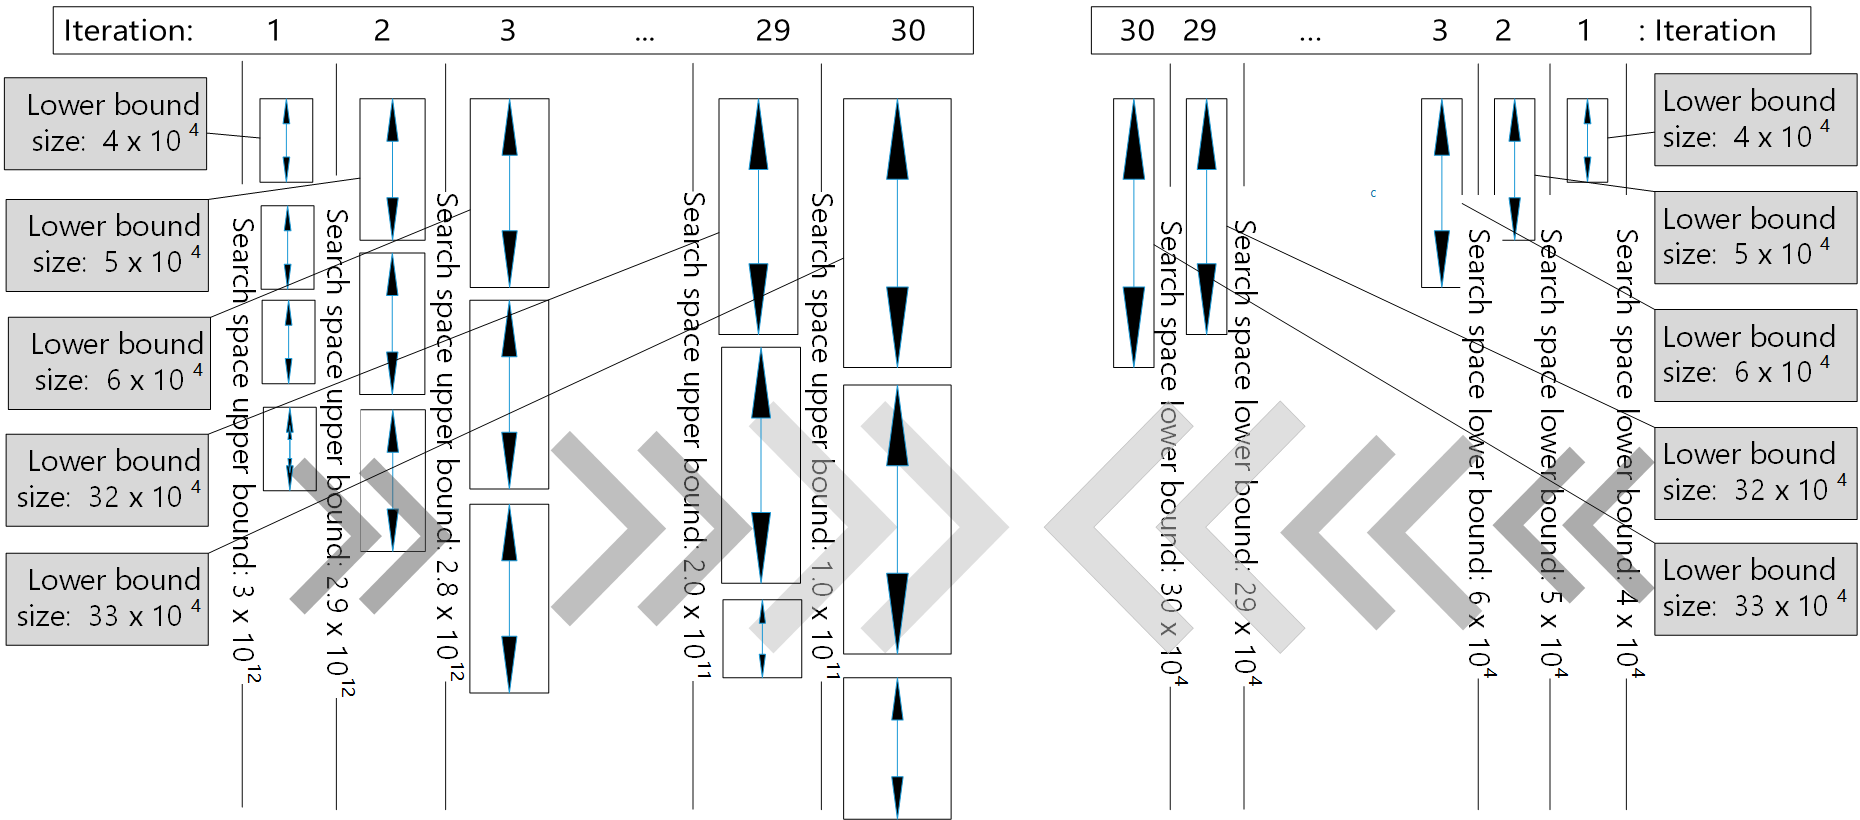
\includegraphics[scale=0.45]{figures/pincer.png}
 	\caption[]{Pincer heuristic}
 	\label{fig:pincer}
 \end{figure}
%
%%%%%%%%%%%%%%%%%%%%%%%%%%%%%%%%%%%%%%%% ALGO 6 %%%%%%%%%%%%%%%%%%%%%%%%%%%%%%%%%%%%%%%%%%
%
\subsection{Backtracking Algorithm} \label{sec:backtracking}

In CSP it is common to find variables that have domain size 1, such variables are designated by singletons. Since both heuristics are based in constraint satisfaction programming, the rotations that we know in advance having variables with domain size 1, are handled first. In case of rotations with schedule maintenance, the algorithm treats them as a flight without turn round time and with the same origin and destination.  Thus when the algorithm creates the aircraft list, the first aircraft have scheduled maintenance. The flights that are disrupted with delays are designated by fixed flights and they too cannot be moved. In this case the domain is a singleton consisting of value \{0\} and if this value is infeasible, because there are no available departure and/or arrival airport capacity, the algorithm backtracks by removing the rotation of an aircraft that can release the necessary airport capacity.

%%%%%%%%%%%%%%%%%%%%%%%%%%%%%%%%%%%%%%% ALGORITHM 6 %%%%%%%%%%%%%%%%%%%%%%%%%%%%%%%%%%%%%%%

Algorithm \ref{algo:backtracking} receives as inputs the singleton list, the airport capacity, the ARP current solution, the rotation nad the index of the first infeasibility. The algorithm will return the ARP solution without the rotation that will allow the singleton to become feasible and, the updated aircraft list. This algorithm will loop while the singleton list is not empty and will verify if the first singleton's infeasibility is on the departure and/or in the arrival airport capacity. Depending on the situation the algorithm computes the airport time slot for the departure/arrival, and based on the origin/destination airport searches the  aircraft to cancel. The algorithm will then remove the aircraft from the solution list, and the respective rotation from the ARP solution. Finally, we will use algorithm \ref{algo:flightDomains} to determine there are any more infeasible singletons.
\begin{algorithm}[H]
	\DontPrintSemicolon
	\KwInput{$ singletonList, \mathcal{A}, aircraftSolList, solutionARP, \sigma_p, index $}
	\KwOutput{$solutionARP, aircraftSolList$}
	\While{$ singletonList \ne \{\}$}{
		
		\If{$singletonList(0) = 'dep'$}{
			$startInt \gets 60 * int(singleton^d(0)/60)$\\
			$endInt \gets startInt + 60$\\
			$origin \gets singleton^o(0)$\\
			$flight2Cancel \gets solutionARP[(origin, startInt, endInt)]$\\
			$airc2Cancel \gets updateMulti(flight2Cancel, \mathcal{A}, solutionARP])$\\
			$aircraftSolList \gets aircraftSolList - airc2Cancel$\\
			$solutionARP.pop(airc2Cancel)$\\
			$flightRanges, singletonList, totalCombos \gets domainFlights(\sigma_p(i) \forall i \in [index, |\sigma_p|], \mathcal{A}, index)$\\
		}
		\If{$singleton(0) = 'arr'$}{
			$startInt \gets 60 * int(singleton^a(0)/60)$\\
			$endInt \gets startInt + 60$\\
			$destination \gets singleton^f(0)$\\
			$flight2Cancel \gets solutionARP[(destination, startInt, endInt)]$\\
			$airc2Cancel \gets updateMulti(flight2Cancel, \mathcal{A}, solutionARP)$\\
			$aircraftSolList \gets aircraftSolList - airc2Cancel$\\
			$solutionARP.pop(airc2Cancel)$\\
			$flightRanges, singletonList, totalCombos \gets domainFlights(\sigma_p(i) \forall i \in [index, |\sigma_p|], \mathcal{A}, index)$\\
		}

	}
	return $solutionARP, aircraftSolList$
	\caption{Backtracking}
	\label{algo:backtracking}
\end{algorithm}

%%%%%%%%%%%%%%%%%%%%%%%%%%%%%%%%%% ALGO 7 %%%%%%%%%%%%%%%%%%%%%%%%%%%%%%%%%%%%%%%%%%
\subsection{Taxi Flights Algorithm} \label{sec:taxiFlights}
After finding a feasible solution for the part of the rotation that was initially infeasible the algorithm tries to reconnect both parts but on occasions it is possible to find discontinuities between them. Algorithm \ref{algo:taxiFlights}  receives as inputs the set of aircraft disruptions, the set of distances, the origin airport, the recovered rotation the maximum flight number and returns the updated recovered rotation and the maximum flight number. Algorithm \ref{algo:taxiFlights} will either create a taxi flight to connect the first part of the rotation and the recovered one, or cancel flights in the recovered rotation until the continuity infeasibility is removed. 

It starts in line 1  initializing the origin slots where there is available departure capacity. Afterwards the algorithm will loop through the flights of the recovered rotation  and if their origin is the same as origin airport it returns the updated recovered rotation and the maximum flight number (lines 2 to 4). In line 5 the algorithm computes the distance from the origin airport and the origin of the flight in the recovered rotation. In line 6 the algorithm extracts the upper slots from the origin slots by subtracting to the flight's departure time in the recovered rotation the distance and the turn round time. In line 7 the upper slots and the aircraft breakdown period are subtracted to the origin slots in order to retrieve the lower slots from where the aircraft can depart. If there are no available departure slots the algorithm cancels the flight in the recovered rotation and continues to the next flight (lines 8 to 10). If there are available departure slots at the origin, the algorithm tries to find destination slots with available airport arrival capacity. To achieve the latter the algorithm finds the destination slots with available capacity, the upper destination slots, and by subtracting the latter to the former and aircraft breakdown period determines the lower destination slots (lines 11 to 13). If there are no lower destination slots, the the algorithm cancels the flight in the recovered rotation and continues to the next flight. Since $\mathcal{A}$ is a dictionary it is necessary to extract the destination intervals and initialize the destination index $i$ and the the time offset from which the flight departs and arrives in feasible airport slots (lines 17 to 21). The algorithm will then loop through the destination slots and in line 23 it will initialize the object $obj$ with the starting and end time of the origin lower slots plus the distance and, in line 24 determine the index of intersection in the destination slot and the offset. If the index $i$ is different from -1 the algorithm will the taxi flight and add it to the recovered rotation (lines 25 to 33).\\ 

\subsection{The CHARP} \label{sec:charp}

In figure \ref{fig:mainAlgo} we provide the complete flowchart of the CHARP. Step 1 of the algorithm consists in loading the data set, after which it starts looping through the aircraft list. In step 2 the algorithm selects an aircraft and it verifies if the rotation has been initialized, if it has not in step 4 and 5 it lists the infeasibilities and adds new flights. If the aircraft's rotation has been initialized in step 6 the algorithm checks if there are infeasibilities and if there are none, in step 10 it updates the ARP's solution with the aircraft's rotation, the airport capacity and the aircraft's solution list. If there are infeasibilities the algorithm will, in step 70, find the flight domains and compute the search space size, after which it will choose solution method (steps 710 and 720) and if necessary the algorithm backtracks.
%%%%%%%%%%%%%%%%%%%%%%%%%%%%%%%%%%%%%%%%%%%%%%%%%%%%%%%%%%%%%%%%%%%%%%
If the size of the search space is lower than the lower bound the algorithm uses the lower heuristic algorithm (step 723), if the search space size is bigger than the upper bound it will use the upper heuristic algorithm (step 713). If neither of the previous apply the algorithm verifies if the loop has finished and if it has not it will move to the next aircraft. After recovering the infeasible part of the rotation the algorithm checks, in step 8, if there is a continuity infeasibility when it tries to reconnect both parts. If there is, in step 9 the taxi flights algorithm reconnects both parts and afterwards adds the recovered rotation to the solution, updates the airport capacity and updates the aircraft solution list (step 10). In step 11  the algorithm checks if the loop has finished aircraft list and if it has it checks if there are any aircraft left to recover (step 12). If there are the algorithm updates the lower and the upper bound and iterates. If there are no more aircraft the algorithm ends.


%%%%%%%%%%%%%%%%%%%%%%%%%%%%%%%%% ALGORITHM 7 %%%%%%%%%%%%%%%%%%%%%%%%%%%%%%%%%%%%%%

\begin{algorithm}[H]
	\DontPrintSemicolon
	\KwInput{$ \mathcal{B},\Delta, originAirport, \sigma_p, \mathcal{A}, M $}
	\KwOutput{$\sigma_p, M$}
	$originSlots \gets \mathcal{A}[originAirport]$ if $capDep > noDep $\\
	\For{$\sigma_p(i)$ in $\sigma_p$}{
		\If{$\sigma^o_p(i) = originAirport$}{
			return $\sigma_p$, M	
		}
		$\delta_{of} \gets \Delta(originAirport, \sigma^{o}_p(i))$\\
		
		$originSlotsUpper \gets  originSlots$ if $endInt > \sigma^d_p(i) - \delta_{of} -t_{rp}$\\
		$originSlotsLower \gets originSlots - originSlotsUpper - [\mathcal{B}^s_p, \mathcal{B}^e_p]$\\
		\If{$originSlotsLower = \{\} $}{
			cancel($\sigma_p(i)$)\\
			continue}
		$destinationSlots \gets \mathcal{A}[\sigma^o_p]$ if $capArr > noArr $\\
		$destinationSlotsUpper \gets  destinationSlots$ if $endInt > \sigma^d_p(i) -t_{rp}$\\
		$destinationSlotsLower \gets destinationSlots - destinationSlotsUpper - [\mathcal{B}^s_p, \mathcal{B}^e_p]$\\
		\If{$destinationSlotsLower = \{\} $}{
			cancel($\sigma_p(i)$)\\
			continue}
		$destIntervals \gets \{\}$\\
		$i \gets -1$\\
		$offset \gets -1$\\
		\For{$x \in destinationSlotsLower$}{
			$destIntervals \gets destIntervals \cup [x^s, x^e]$
		}
		\For{$os(i)$ in $originSlotsLower$}{
			$obj \gets interval(os^s, os^e) + distInitRot$\\
			$i, offset \gets obj.findIntersection(destIntervals)$\\
			\If{$i \ne -1$}{	
				$taxiFlight^o \gets originAirport$\\
				$taxiFlight^d \gets os['startInt'] + offset$\\
				$taxiFlight^f = \sigma^o_p(i)$\\
				$taxiFlight^a = taxiFlight^d + \delta_{of}$\\
				$taxiFlight['flight'] = M$\\
				$M \gets M + 1$\\
				$\sigma_p \gets \sigma_p + taxiFlight$\\
				return $\sigma_p, M$\\}
		}
	}
	\label{algo:taxiFlights}
	\caption{Taxi flights}
\end{algorithm}


 \begin{figure}[h!]
	\centering
	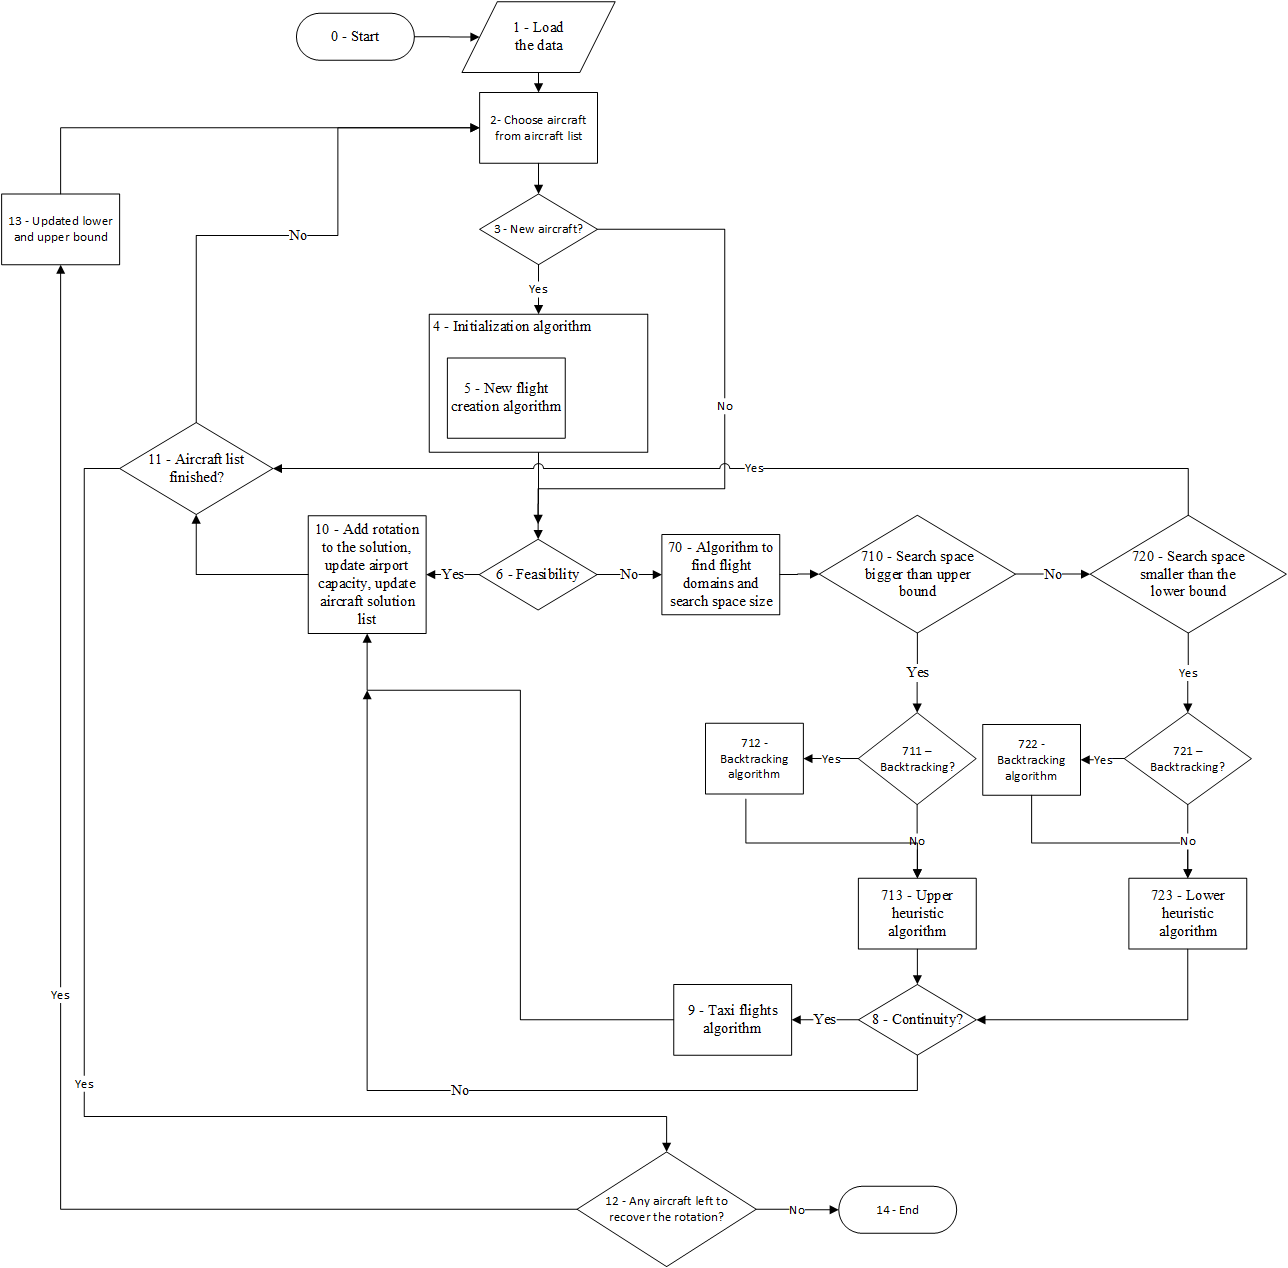
\includegraphics[scale=0.65]{figures/mainAlgo.png}
	\caption[]{Constructive heuristic}
	\label{fig:mainAlgo}
\end{figure}

%\end{document}
